\documentclass{article}
\usepackage[utf8]{inputenc}

\title{Principal Component Analysis (PCA)}
\author{Tara Mirmira }
\date{July 2017}

\usepackage{natbib}
\usepackage{graphicx}
\usepackage{amsmath}

\begin{document}

\maketitle

\section{Problem}
We want to build a linear model for the variable $\boldsymbol{y}$ using the explanatory variables $\boldsymbol{x_1}, \ldots, \boldsymbol{x_p}$. The coefficient for the explanatory variable $x_j$ is $\hat{\boldsymbol{\beta_j}}$. The standard error for the coefficient is:
$$
SE(\hat{\boldsymbol{\beta_j}}) = \dfrac{1}{\sqrt{1 - {R_j}^2}}\dfrac{\sigma}{\sqrt{\sum_{i=1}^n (x_{ji} - \overline{x_j})^2}}
$$
where
\begin{itemize}
    \item $R$ is the multiple correlation coefficient from regressing $\boldsymbol{x_j}$ on the other explanatory variables $\boldsymbol{x_1}, \ldots, \boldsymbol{x_{j-1}}, \boldsymbol{x_{j+1}}, \ldots, \boldsymbol{x_p}$
    \item $n$ is the number of observations in the data set
    \item $\sigma$ is the standard deviation of the residuals from fitting the full model to the data
    \item $Var(x_{ji}) = \frac{1}{n-1}\sum_{i=1}^n (x_{ji} - \overline{x_j})^2$ so $\sum_{i=1}^n (x_{ji} - \overline{x_j})^2 = (n-1)*Var(x_{ji})$
\end{itemize}

If the explanatory variables are collinear, the fit from regressing $\boldsymbol{x_j}$ on the other explanatory variables improves, which means $R_j$ becomes larger. When $R_j$ increases, the term $\frac{1}{\sqrt{1-{R_j}^2}}$, also called the Variance Inflation Factor (VIF), increases so $SE(\hat{\boldsymbol{\beta_j}})$ increases. As the variance of the coefficients increases, the the coefficients become unstable, meaning they can vary greatly. In the most extreme case where one explanatory variable is perfectly collinear with another, there is no unique solution $\boldsymbol{\hat{\beta}}$ for the coefficients.

\section{Solution}

To remedy the problem described above, we will try to find a new set of vectors $\boldsymbol{W} = \{\boldsymbol{w_1}, \ldots, \boldsymbol{w_p}\}$ that spans the same vector space as the columns of the design matrix $\boldsymbol{X}$. Recall that  
$$
\boldsymbol{X} = \begin{bmatrix}
    \boldsymbol{1}       & \boldsymbol{x_1} & \dots & \boldsymbol{x_p}
\end{bmatrix}
$$

\noindent We will replace the design matrix $\boldsymbol{X}$ with $\boldsymbol{W}$ to build the model. The $\boldsymbol{w_i} \in \boldsymbol{W}$ are called principal components. There are two special features about the vectors in $\boldsymbol{W}$:
\begin{itemize}
    \item The vectors are orthogonal
    \item The vectors are in order of decreasing variance for their respective coefficient. This means: 
    \begin{itemize}
        \item The coefficient for $\boldsymbol{w_1}$ has the greatest variance 
        \item The coefficient for $\boldsymbol{w_p}$ has the smallest variance
    \end{itemize}
\end{itemize}

\begin{figure}[hbtp]
        \centering
        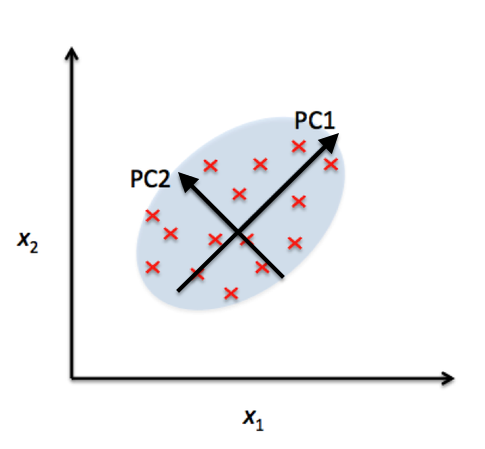
\includegraphics[width=4.5in]{pca.png}
        \caption{principal Components Diagram}
        \label{Newton Raphson}
    \end{figure}

\noindent In the above picture, we can see that the two principal components are orthogonal. The first component, PC1, covers more spread, showing that PC1 has the greatest variability. In two dimensions, PC1 is the major axis of an ellipse and PC2 is the minor axis.

\section{How to Find $\boldsymbol{W}$}

Note: the method described here is not efficient for data with many explanatory variables (large $p$). 

\begin{enumerate}
    \item Standardize the data. 
    $$
    \boldsymbol{X} = 
    \begin{bmatrix}
    \boldsymbol{x_1} & \dots & \boldsymbol{x_p}
\end{bmatrix} \rightarrow 
\boldsymbol{Z} = 
    \begin{bmatrix}
    \boldsymbol{z_1} & \dots & \boldsymbol{z_p}
\end{bmatrix} 
    $$
    
    $$
    \text{where } \boldsymbol{z_i} = \frac{\boldsymbol{x_i} - \overline{x_i}\boldsymbol{1}}{SD(x_i)\boldsymbol{1}} \text{and} SD(x_i) = \sqrt{\frac{1}{n-1}\sum_{j=1}^n (x_ij - \overline{x_i})^2}
    $$
    
   If the original data had variances that are very different, we will lean towards including the variables with larger variances in the first few principal components. To eliminate this effect, the data should first be standardized.
   
   \item Find a new set of basis vectors for $span\{\boldsymbol{z_1}, \ldots, \boldsymbol{z_p}\}$ 

    The first principal component $\boldsymbol{w_1}$ can be written as a linear combination of the $\boldsymbol{z_i}'s$. 
    $$
    \boldsymbol{w_1} = a_{11}\boldsymbol{z_1} + a_{12}\boldsymbol{z_2} + \ldots + a_{1p}\boldsymbol{z_p}
    $$
    
    \noindent We want to find the $a_{1i}'s$ such that $Var(\boldsymbol{w_1})$ is the greatest of all the $\boldsymbol{w_i}'s$.\\
    
    $\overline{\boldsymbol{w_1}} = 0$ because all the $\boldsymbol{z_i}'s$ have mean $0$ since they have been standardized\\
    
    $$Var(\boldsymbol{w_1}) = \frac{1}{n-1}\sum_{i=1}^n (w_{1i} - \overline{\boldsymbol{w_1}})^2 = \frac{1}{n-1}\sum_{i=1}^n w_{1i}^2 = \frac{1}{n-1}\boldsymbol{w_1^T w_1}$$
    


Calculations:

$$
\boldsymbol{Z^T}\boldsymbol{Z} = 
\begin{bmatrix}
\sum z_{1i}^2 & \sum z_{1i}z_2i & \ldots \\
\sum z_{2i}z_{1i} & \sum z_{2i}^2 & \ldots \\
\vdots & \vdots & \ddots \\
\end{bmatrix}
$$

$\sum z_{1i}^2 = \dfrac{\sum (x_{1i} - \overline{x_1})^2}{s_1^2}$ \\

$\frac{1}{n-1}\sum z_{1i}^2 = \frac{1}{n-1}\dfrac{\sum (x_{1i} - \overline{x_1})^2}{s_1^2} = 1$ because $\boldsymbol{z_1}$ is standardized $\boldsymbol{x_1}$

Using the above calculation:

$$
\frac{1}{n-1}\boldsymbol{Z^T}\boldsymbol{Z} = 
\begin{bmatrix}
1 & r_{12} & \ldots & r_{1p}\\
r_{21} & 1 & \ldots & r_{2p}\\
\vdots & \vdots & \ddots \\
r_{p1} & r_{p2} & \ldots & 1 \\
\end{bmatrix} = \boldsymbol{R_{xx}} \text{ (the correlations of the $\boldsymbol{x_i}'s$)}
$$

where $$r_{ij} = \frac{1}{n-1}\sum_{k=1}^n \frac{z_{ik} - \overline{z_i}}{SD(z_i)}\frac{z_{jk} - \overline{z_j}}{SD(z_j)} = \frac{1}{n-1}\sum_{k=1}^n \frac{z_{ik} - 0}{1}\frac{z_{jk} - 0}{1} = \frac{1}{n-1}\sum_{k=1}^n z_{ik}z_{jk}$$ is the correlation coefficient between $\boldsymbol{z_i}$ and $\boldsymbol{z_j}$\\

\noindent Note that $\boldsymbol{R_{xx}}$ is also the Variance-Covariance matrix for the matrix $\boldsymbol{Z}$.
\\\\
$
\max_{\boldsymbol{a_1}} (\boldsymbol{a_1}^t\boldsymbol{R_{xx}}\boldsymbol{a_1}) \text{ where } \boldsymbol{a_1}^t\boldsymbol{a_1} = 1 \quad (1)
$
\\\\
\noindent We include the constraint $\boldsymbol{a_1}^t\boldsymbol{a_1} = 1$ so that when taking the maximum with respect to $\boldsymbol{a_1}$, $\boldsymbol{a_1}$ does not increase to infinity.\\\\

\noindent Equation $(1)$ above is equivalent to:\\\\

$\max_{\boldsymbol{a_1}, \lambda} \boldsymbol{a_1}^t\boldsymbol{R_{xx}}\boldsymbol{a_1} - \lambda(\boldsymbol{a_1}^t\boldsymbol{a_1} - 1)$\\\\

\noindent Taking the derivative with respect to $\boldsymbol{a_1}$:\\\\

$
2\boldsymbol{R_{xx}} - 2\lambda \boldsymbol{a_1} = 0
$\\\\

$
\boldsymbol{R_{xx}a_1} = \lambda \boldsymbol{a_1}
$
\\\\
What the above calculation shows is that the principal components are the eigenvectors of the matrix $\boldsymbol{R_{xx}}$. The first principal component is the eigenvector corresponding to the largest eigenvector. We order the eigenvalues $\lambda_1 \geq \lambda_2 \geq \ldots \geq \lambda_p > 0$ and the corresponding eigenvectors $\boldsymbol{w_1}, \ldots, \boldsymbol{w_p}$ are the orthogonal principal components in order of decreasing variance.

\item Find the eigenvectors and eigenvalues of $\boldsymbol{R_{xx}}$, the variance-covariance matrix for $\boldsymbol{Z}$.
\end{enumerate}

Summary of the calculations and steps:
\begin{enumerate}
    \item Standardize the input: $\boldsymbol{X} \rightarrow \boldsymbol{Z}$
    \item Find the $\boldsymbol{R_{xx}}$, the variance-covariance matrix for $\boldsymbol{Z}$
    \item Find the eigenvectors and eigenvalues of $\boldsymbol{R_{xx}}$
\end{enumerate}

\end{document}
